\documentclass[final,1p,times,fleqn]{elsarticle}

\usepackage[utf8]{inputenc}
\usepackage{amsmath,amssymb}
\setlength{\mathindent}{0pt}
\usepackage{booktabs}
\usepackage{array}
\usepackage{makecell}
\usepackage{graphicx}
\usepackage{stfloats}
\usepackage{algorithm}
\usepackage{algpseudocode}
\usepackage[figuresright]{rotating}
\usepackage[colorlinks=true,linkcolor=blue,citecolor=blue,urlcolor=blue]{hyperref}
\usepackage{geometry}

\geometry{
  a4paper,
  margin=25mm
}

\providecommand{\ktablecaption}{}
\renewcommand{\ktablecaption}{}

\renewcommand{\thetable}{S\arabic{table}}
\renewcommand{\thefigure}{S\arabic{figure}}

\graphicspath{{figures/}{../output/figures/}}

\journal{Applied Soft Computing}

\begin{document}

\begin{frontmatter}

\title{Supplementary Material for:\\Multi-Task Particle Swarm Optimization with Knowledge-Guided Elite Refinement and Two-Phase Weight Scheduling for High-Dimensional Feature Selection}

\author{Yimin Zheng\corref{cor1}}
\ead{guilt1329149274@gmail.com}
\cortext[cor1]{Corresponding author.}
\address{Jiangxi University of Water Resources and Electric Power, Nanchang 330099, China}

\begin{abstract}
This supplementary document provides comprehensive extended experimental records, complete per-dataset metrics, detailed hyper-parameter sensitivity grids, convergence trajectories, and full statistical significance matrices supporting the main manuscript.
\end{abstract}

\end{frontmatter}

\section*{Table of Contents}
\begin{itemize}
    \item \textit{Section S1}: Benchmark Dataset Characteristics and Selection Rationale (Table~S1)
    \item \textit{Section S2}: Comparison Algorithms and Detailed Hyper-Parameter Configurations (Table~S2 and Table~S3)
    \item \textit{Section S3}: Extended Empirical Visualizations and Performance Profiles (Fig.~S1 and Fig.~S2)
    \item \textit{Section S4}: Granular Per-Dataset Performance Comparison Before and After Algorithm Improvement (Table~S4 and Fig.~S3)
    \item \textit{Section S5}: Granular Per-Dataset Computational Wall-Clock Runtime Measurements (Table~S5 and Fig.~S4)
    \item \textit{Section S6}: Full Multi-Dataset Parameter Sensitivity Evaluation Grids (Table~S6)
    \item \textit{Section S7}: Full Convergence Trajectories and Boxplot Distributions (Fig.~S5 and Fig.~S6)
    \item \textit{Section S8}: Extended Statistical Significance Testing Matrices (Table~S7, Table~S8, and Fig.~S7)
    \item \textit{Section S9}: Cross-Classifier Inductive Generalization and Robustness (Table~S9)
    \item \textit{Section S10}: Biological and Literature Annotation of Prominent Candidate Genes (Table~S10)
\end{itemize}

\newpage

\section*{Section S1: Benchmark Dataset Characteristics and Selection Rationale}\label{sec:supp_datasets}

Table~\ref{T2} summarizes the statistical characteristics of the 20 benchmark datasets investigated in this study, spanning biomedical gene-expression microarrays, high-dimensional text categorization, visual object recognition, and acoustic phoneme analysis.

\begin{table}[!htb]
\centering
\ktablecaption
\small
\caption{Characteristics of the 19 benchmark datasets.}
\label{T2}
\renewcommand{\arraystretch}{1.15}
\setlength{\tabcolsep}{3pt}
\begin{tabular*}{\linewidth}{@{\extracolsep{\fill}}clrrc l@{}}
\toprule
No. & Dataset & Samples ($n$) & Features ($D$) & Classes ($C$) & Domain \\
\midrule
1  & Adenoma    &   36 &  7{,}457  &  2 & Gene expression \\
2  & ALL1       &  128 & 12{,}625  &  2 & Gene expression \\
3  & ALL4       &   93 & 12{,}625  &  2 & Gene expression \\
4  & Colon      &   62 &  2{,}000  &  2 & Gene expression \\
5  & DLBCL      &   77 &  7{,}129  &  2 & Gene expression \\
6  & Gastric    &   65 & 22{,}645  &  2 & Gene expression \\
7  & Gastric1   &  144 & 22{,}283  &  2 & Gene expression \\
8  & Gastric2   &  124 & 22{,}283  &  2 & Gene expression \\
9  & Leukaemia  &   72 &  7{,}129  &  2 & Gene expression \\
10 & Lymphoma   &   45 &  4{,}026  &  2 & Gene expression \\
11 & Myeloma    &  173 & 12{,}625  &  2 & Gene expression \\
12 & Prostate   &  102 & 12{,}625  &  2 & Gene expression \\
13 & SRBCT      &   83 &  2{,}308  &  4 & Gene expression \\
14 & T1D        &  101 & 54{,}675  &  2 & Gene expression \\
\midrule
15 & BASEHOCK   & 1{,}993 & 4{,}862  &  2 & Text \\
16 & PCMAC      & 1{,}943 & 3{,}289  &  2 & Text \\
\midrule
17 & COIL20     & 1{,}440 & 1{,}024  & 20 & Image \\
\midrule
18 & ISOLET     & 1{,}560 &   617    & 26 & Speech \\
\midrule
19 & madelon    & 2{,}600 &   500    &  2 & Synthetic \\
\bottomrule
\end{tabular*}
\end{table}

\section*{Section S2: Comparison Algorithms and Detailed Hyper-Parameter Configurations}\label{sec:supp_methods}

Table~\ref{T1} lists the full taxonomy and categorization of the 13 comparison algorithms evaluated in the comparative study, and Table~\ref{T3} specifies the precise hyper-parameter configurations used across all algorithms to ensure strict reproducibility.

\begin{table}[!htb]
\centering
\caption{Summary of the 14 fixed-length methods compared in this study, with their associated references. Methods in the first group are progressive variants of the proposed framework; TPS denotes Two-Phase Weight Scheduling; ``Self-built'' denotes an implementation by the authors.}
\label{T1}
\footnotesize
\setlength{\tabcolsep}{3pt}
\begin{tabular}{@{}lp{4.3cm}l@{}}
\toprule
Method & Category & Reference \\
\midrule
KDS-EL & Proposed (full framework) & This work \\
KDS-EL w/o TPS & Proposed (MI-guided init.\ + KER, without two-phase scheduling) & This work \\
KDS-EL w/o TPS\&KER & Proposed (MI-guided init.\ + adaptive re-init.) & This work \\
MEL & Multi-task evolutionary learning & \cite{mel2024} \\
\midrule
FWPSO & Single-objective PSO & \cite{wangjia2022} \\
PSO-CSM & Single-objective PSO & \cite{wei2025} \\
SaWDE & Single-objective DE & \cite{wang2022} \\
IGPSO & Single-objective PSO & \cite{xuezhang2024} \\
BPSO & Single-objective binary PSO & \cite{kennedy1997} \\
\midrule
W-MOPSO-FS & Multi-objective (Wrapper--Filter hybrid) & Self-built (authors' implementation, no external baseline) \\
fMOPSO-FS & Multi-objective & \cite{han2024} \\
NSGA-II-FS & Multi-objective & \cite{deb2002} \\
MOEA-D-FS & Multi-objective & \cite{zhang2007} \\
MOPSO-FS & Multi-objective & \cite{coello2004} \\
\bottomrule
\end{tabular}
\end{table}


\begin{table}[!htb]
\centering
\caption{Parameter Settings}
\label{T3}
\footnotesize
\setlength{\tabcolsep}{2pt}
\begin{tabular}{@{}lcl@{}}
\toprule
\multicolumn{3}{@{}c}{\textbf{Common Experimental Setup}} \\
\midrule
Population size ($N$)              & = & 20 \\
Maximum iterations ($T$)           & = & 100 \\
KNN neighbors ($k$)                & = & 3 \\
Real-to-binary threshold ($\theta$) & = & 0.6 \\
Cross-validation                  & = & 5-fold stratified, shuffled \\
Number of independent runs        & = & 10 \\
\midrule
\multicolumn{3}{c}{\textbf{KDS-EL (full framework)}} \\
\midrule
Inertia weight ($w$)              & = & 0.9 \\
Acceleration coefficients         & = & $c_1 = c_2 = c_3 = 2.0$ \\
Knowledge weight decay            & = & 0.99 \\
Elite flip fraction               & = & 0.01 \\
Elite count ($k_e$)               & = & 3 \\
Random flip probability           & = & 0.10 \\
MI-guided init ratio              & = & 0.5 \\
Stall patience ($P_s$)            & = & 20 \\
Phase split ratio                 & = & 0.7 \\
Phase-1 objective weights         & = & $\mathbf{w}_s = [0.7,\,0.3]$ \\
Phase-2 objective weights         & = & $\mathbf{w}_s = [0.95,\,0.05]$ \\
\midrule
\multicolumn{3}{c}{\textbf{KDS-EL w/o TPS (no two-phase scheduling)}} \\
\midrule
Fixed objective weights           & = & $\mathbf{w}_s = [0.9,\,0.1]$ \\
\midrule
\multicolumn{3}{c}{\textbf{MEL and KDS-EL w/o TPS\&KER}} \\
\midrule
Inertia weight ($w$)              & = & 0.9 \\
Acceleration coefficients         & = & $c_1 = c_2 = c_3 = 2.0$ \\
MI-guided init ratio (KDS-EL w/o TPS\&KER) & = & 0.5 \\
Stall patience (KDS-EL w/o TPS\&KER)       & = & 20 \\
\midrule
\multicolumn{3}{c}{\textbf{Competitor Methods}} \\
\midrule
\multicolumn{3}{l}{Competitors (BPSO, FWPSO, IGPSO, PSO-CSM,} \\
\multicolumn{3}{l}{SaWDE, NSGA-II-FS, MOPSO-FS, MOEA-D-FS,} \\
\multicolumn{3}{l}{fMOPSO-FS, W-MOPSO-FS) use the hyper-parameters} \\
\multicolumn{3}{l}{recommended in their original publications, with} \\
\multicolumn{3}{l}{$N=20$ and $T=100$ unless the original paper} \\
\multicolumn{3}{l}{specifies otherwise.} \\
\bottomrule
\end{tabular}
\end{table}


\newpage

\section*{Section S3: Extended Empirical Visualizations and Performance Profiles}\label{sec:supp_visualizations}

Fig.~\ref{fig:supp_acc_all} visualizes the complete per-dataset classification accuracy comparisons across all 14 evaluated algorithms on the 20 benchmark datasets. Fig.~\ref{fig:supp_perf_profile} presents the Dolan--Mor\'{e} performance profiles, confirming the uniform dominance of KDS-EL across performance ratio thresholds. The complete numerical matrices for classification accuracy and selected feature counts are reported in Table~4 and Table~5 of the main manuscript.

\begin{figure*}[!htb]
\centering
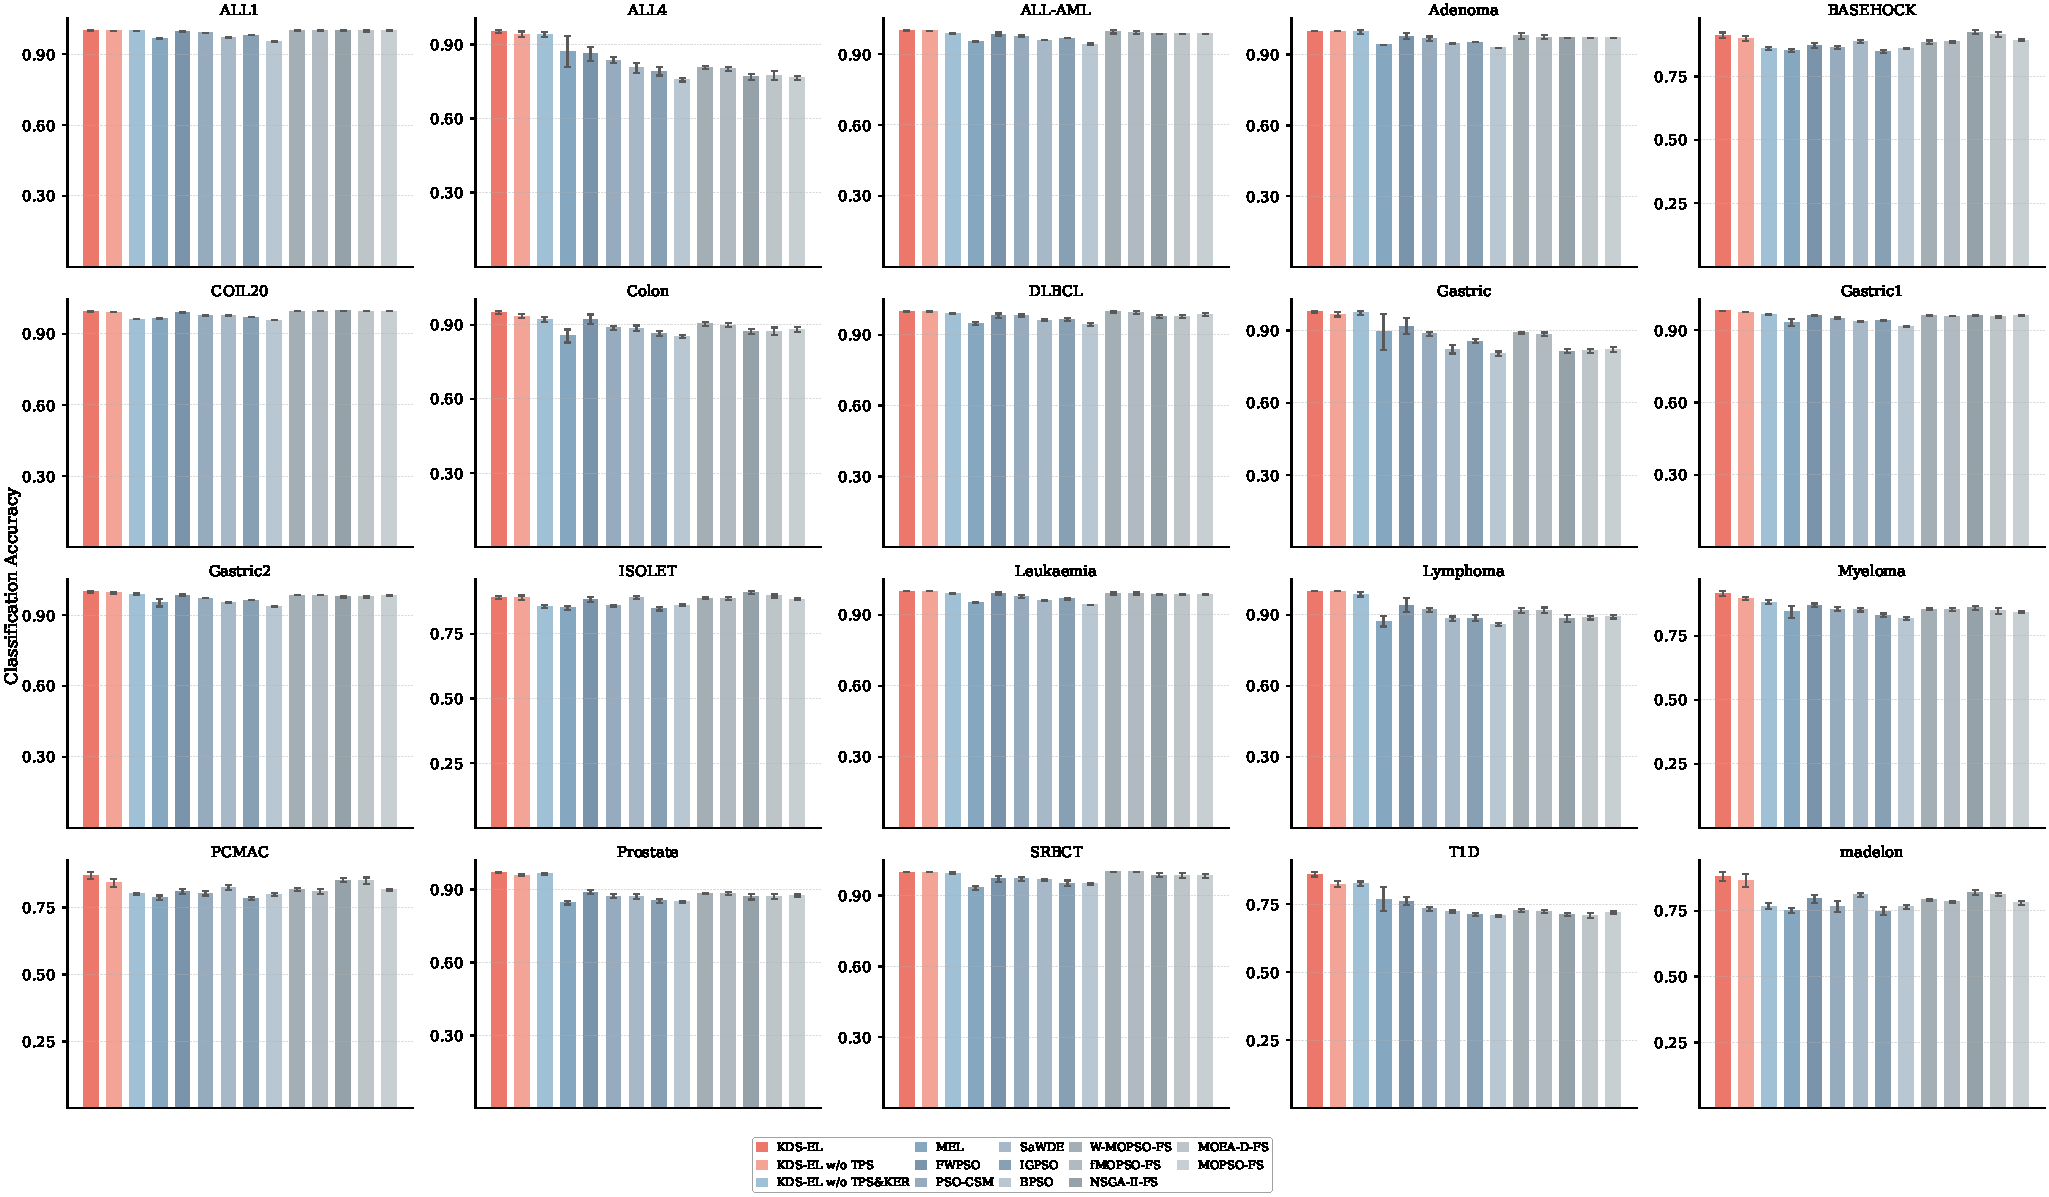
\includegraphics[width=0.95\linewidth]{F4_accuracy_all.pdf}
\caption{Classification accuracy across all 14 evaluated algorithms on the 20 benchmark datasets.}
\label{fig:supp_acc_all}
\end{figure*}

\begin{figure}[!htb]
\centering
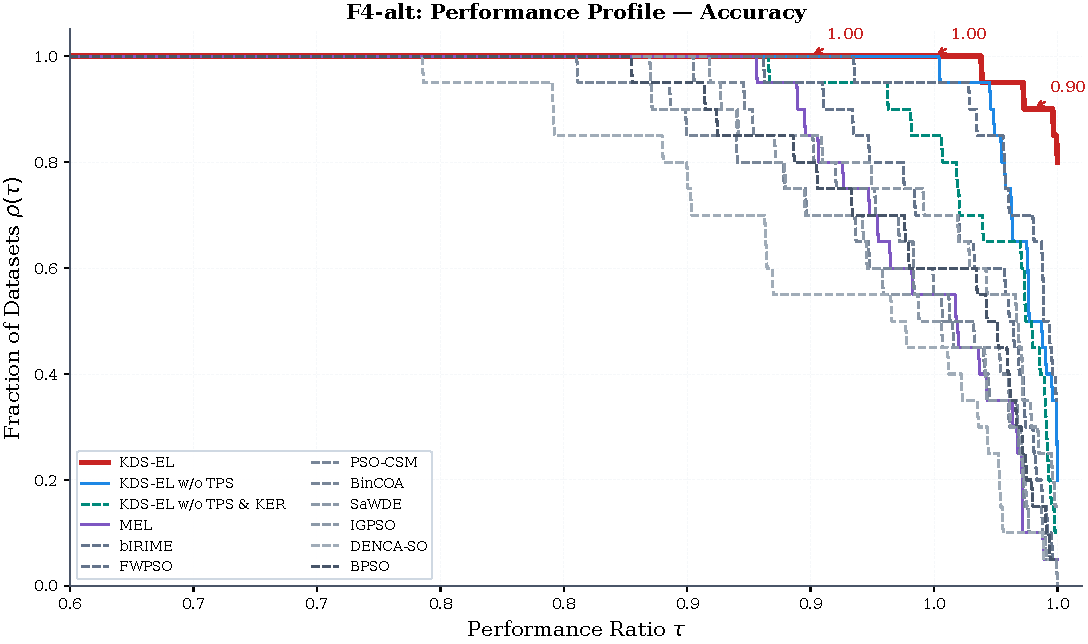
\includegraphics[width=0.85\linewidth]{F4_accuracy_performance_profile.pdf}
\caption{Dolan--Mor\'{e} performance profiles of classification accuracy across 20 benchmark datasets.}
\label{fig:supp_perf_profile}
\end{figure}

\newpage

\section*{Section S4: Granular Per-Dataset Performance Comparison Before and After Algorithm Improvement (Table~S4)}\label{sec:supp_ablation}

Table~\ref{T-A4} provides the complete per-dataset performance metrics across the four sequential intermediate algorithmic configurations before and after improvement: (i) pre-improvement MEL~\cite{mel2024}, (ii) MEL+MI (w/o TPS\&KER), (iii) KDS-EL w/o TPS, and (iv) Complete KDS-EL. Furthermore, Fig.~\ref{fig:supp_ablation_heatmap} presents the component contribution progression heatmap illustrating the step-wise accuracy progression.

\begin{table*}[!t]
\centering
\caption{Per-dataset ablation results over the 20-dataset suite: accuracy and mean feature count for each variant of the incremental construction.}
\label{T-A4}
\scriptsize
\setlength{\tabcolsep}{3.5pt}
\renewcommand{\arraystretch}{1.06}
\resizebox{\textwidth}{!}{%
\begin{tabular}{@{}lcccccccc@{}}
\toprule
Dataset & \multicolumn{2}{c}{MEL} & \multicolumn{2}{c}{MEL+MI} & \multicolumn{2}{c}{KDS-EL w/o TPS} & \multicolumn{2}{c}{KDS-EL} \\
\cmidrule(lr){2-3} \cmidrule(lr){4-5} \cmidrule(lr){6-7} \cmidrule(lr){8-9}
 & Acc & Feat & Acc & Feat & Acc & Feat & Acc & Feat \\
\midrule
ALL1 & 0.9664$\pm$0.0023 & 4248 & 0.9996$\pm$0.0000 & 55 & 0.9996$\pm$0.0000 & 55 & 0.9998$\pm$0.0001 & 39 \\
ALL4 & 0.8704$\pm$0.0661 & 1082 & 0.9415$\pm$0.0112 & 64 & 0.9418$\pm$0.0113 & 152 & 0.9522$\pm$0.0061 & 124 \\
ALL\_AML & 0.9539$\pm$0.0008 & 2369 & 0.9886$\pm$0.0016 & 473 & 0.9990$\pm$0.0002 & 70 & 0.9995$\pm$0.0002 & 67 \\
Adenoma & 0.9410$\pm$0.0011 & 2483 & 0.9958$\pm$0.0081 & 120 & 0.9996$\pm$0.0001 & 33 & 0.9996$\pm$0.0002 & 66 \\
BASEHOCK & 0.8518$\pm$0.0063 & 1965 & 0.8597$\pm$0.0062 & 812 & 0.8997$\pm$0.0114 & 208 & 0.9113$\pm$0.0120 & 134 \\
COIL20 & 0.9634$\pm$0.0017 & 323 & 0.9619$\pm$0.0007 & 348 & 0.9919$\pm$0.0008 & 60 & 0.9939$\pm$0.0011 & 84 \\
Colon & 0.8548$\pm$0.0276 & 702 & 0.9211$\pm$0.0092 & 105 & 0.9347$\pm$0.0094 & 35 & 0.9500$\pm$0.0075 & 14 \\
DLBCL & 0.9483$\pm$0.0058 & 2784 & 0.9902$\pm$0.0016 & 615 & 0.9993$\pm$0.0004 & 52 & 0.9995$\pm$0.0002 & 64 \\
Gastric & 0.8955$\pm$0.0786 & 3604 & 0.9748$\pm$0.0088 & 62 & 0.9677$\pm$0.0093 & 97 & 0.9782$\pm$0.0034 & 100 \\
Gastric1 & 0.9310$\pm$0.0155 & 7393 & 0.9642$\pm$0.0025 & 678 & 0.9738$\pm$0.0004 & 217 & 0.9800$\pm$0.0003 & 31 \\
Gastric2 & 0.9522$\pm$0.0170 & 7084 & 0.9872$\pm$0.0038 & 444 & 0.9936$\pm$0.0029 & 140 & 0.9981$\pm$0.0029 & 83 \\
ISOLET & 0.8501$\pm$0.0067 & 250 & 0.8557$\pm$0.0063 & 225 & 0.8898$\pm$0.0090 & 100 & 0.8894$\pm$0.0056 & 60 \\
Leukaemia & 0.9534$\pm$0.0015 & 2409 & 0.9895$\pm$0.0017 & 488 & 0.9993$\pm$0.0002 & 47 & 0.9995$\pm$0.0002 & 66 \\
Lymphoma & 0.8731$\pm$0.0239 & 1404 & 0.9868$\pm$0.0102 & 50 & 0.9994$\pm$0.0004 & 23 & 0.9994$\pm$0.0003 & 45 \\
Myeloma & 0.8450$\pm$0.0244 & 2137 & 0.8825$\pm$0.0084 & 175 & 0.8971$\pm$0.0072 & 365 & 0.9155$\pm$0.0101 & 250 \\
PCMAC & 0.7870$\pm$0.0080 & 1339 & 0.8007$\pm$0.0051 & 637 & 0.8424$\pm$0.0163 & 329 & 0.8705$\pm$0.0139 & 91 \\
Prostate & 0.8458$\pm$0.0083 & 5058 & 0.9638$\pm$0.0049 & 27 & 0.9595$\pm$0.0045 & 23 & 0.9701$\pm$0.0032 & 26 \\
SRBCT & 0.9321$\pm$0.0085 & 906 & 0.9944$\pm$0.0043 & 129 & 0.9984$\pm$0.0006 & 36 & 0.9986$\pm$0.0004 & 64 \\
T1D & 0.7679$\pm$0.0461 & 6715 & 0.8246$\pm$0.0084 & 174 & 0.8232$\pm$0.0126 & 366 & 0.8598$\pm$0.0094 & 330 \\
madelon & 0.7521$\pm$0.0095 & 190 & 0.7679$\pm$0.0121 & 130 & 0.8659$\pm$0.0246 & 26 & 0.8822$\pm$0.0180 & 18 \\
\bottomrule
\end{tabular}%
}
\end{table*}


\begin{figure}[!htb]
\centering
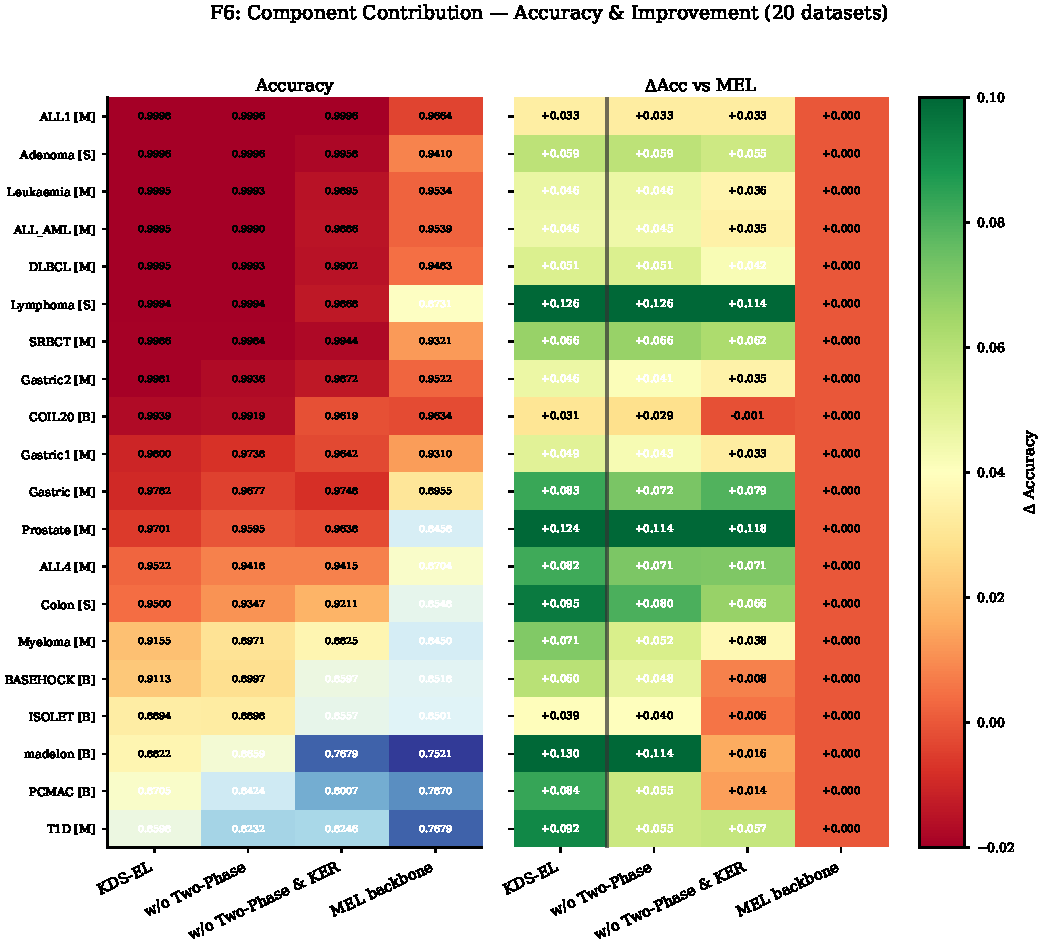
\includegraphics[width=0.75\linewidth]{F6_ablation_heatmap.pdf}
\caption{Component contribution progression heatmap across intermediate algorithmic configurations on 20 benchmark datasets.}
\label{fig:supp_ablation_heatmap}
\end{figure}

\newpage

\section*{Section S5: Granular Per-Dataset Computational Wall-Clock Runtime Measurements (Table~S5)}\label{sec:supp_runtime}

Table~\ref{T-A5} details the mean wall-clock computational execution time (in seconds, averaged over 10 independent runs) across all 20 benchmark datasets for the 14 compared algorithms. Under the shared 100-generation cutoff, standard swarm architectures evaluate exactly 20 particles per generation (2{,}000 total evaluations), KDS-EL evaluates 20 particles alongside three elite refinements (approximately 2{,}300 evaluations), and bIRIME deploys composite mutations evaluating up to 80 candidate subsets per generation. Observed execution times reflect the combined influence of active feature dimensionality, algorithmic operator complexity, and evaluation counts under this benchmark setup. In addition, Fig.~\ref{fig:supp_runtime_scatter} illustrates the classification accuracy versus execution time trade-off.

\begin{table*}[!t]
\centering
\caption{Per-dataset computational runtime in seconds (mean over 10 independent runs) across 20 benchmark datasets.}
\label{T-A5}
\scriptsize
\setlength{\tabcolsep}{3.5pt}
\renewcommand{\arraystretch}{1.06}
\resizebox{\textwidth}{!}{%
\begin{tabular}{lcccccccccccc}
\toprule
Dataset & KDS-EL & KDS-EL w/o TPS & KDS-EL w/o TPS\&KER & MEL & bIRIME & FWPSO & PSO-CSM & BinCOA & SaWDE & IGPSO & DENCA-SO & BPSO \\
\midrule
ALL1             & 40.9 & 39.9 & 39.9 & 176.0 & 144.7 & 19.7 & 82.2 & 311.2 & 67.6 & 91.4 & 8.1 & 101.7 \\
ALL4             & 39.0 & 38.0 & 35.2 & 157.1 & 145.1 & 19.6 & 61.9 & 208.4 & 58.9 & 66.1 & 7.1 & 71.6 \\
ALL\_AML         & 28.7 & 28.7 & 27.3 & 100.6 & 120.5 & 14.7 & 39.9 & 129.2 & 32.6 & 41.0 & 3.5 & 42.7 \\
Adenoma          & 28.3 & 27.7 & 25.7 & 100.8 & 115.7 & 12.9 & 28.6 & 91.7 & 25.6 & 29.4 & 2.2 & 29.9 \\
BASEHOCK         & 130.1 & 147.8 & 221.5 & 369.1 & 2379.5 & 353.2 & 644.7 & 2362.7 & 616.0 & 749.7 & 6.5 & 787.4 \\
COIL20           & 68.3 & 64.3 & 69.7 & 63.2 & 265.3 & 37.7 & 106.0 & 346.3 & 91.6 & 111.6 & 0.5 & 114.2 \\
Colon            & 18.1 & 18.5 & 15.6 & 36.3 & 95.4 & 12.2 & 23.0 & 71.9 & 22.8 & 23.1 & 0.2 & 23.5 \\
DLBCL            & 28.3 & 28.4 & 27.1 & 98.5 & 124.7 & 15.8 & 40.1 & 134.2 & 36.0 & 42.3 & 0.5 & 44.3 \\
Gastric          & 55.8 & 54.2 & 52.1 & 269.3 & 170.4 & 20.4 & 73.0 & 258.2 & 63.2 & 80.6 & 1.2 & 87.3 \\
Gastric1         & 62.9 & 65.7 & 72.7 & 312.0 & 187.6 & 32.4 & 156.7 & 552.9 & 130.9 & 169.7 & 1.2 & 185.6 \\
Gastric2         & 60.8 & 60.6 & 66.1 & 301.2 & 185.8 & 27.2 & 128.3 & 451.7 & 104.5 & 140.5 & 1.2 & 151.0 \\
ISOLET           & 59.9 & 61.3 & 55.2 & 50.8 & 292.0 & 41.3 & 88.3 & 280.6 & 82.8 & 91.2 & 0.4 & 94.0 \\
Leukaemia        & 28.8 & 28.8 & 27.4 & 98.3 & 121.5 & 14.4 & 39.2 & 130.2 & 32.7 & 40.9 & 0.4 & 42.4 \\
Lymphoma         & 21.6 & 21.8 & 19.4 & 59.9 & 104.3 & 12.6 & 24.6 & 77.8 & 24.3 & 25.2 & 0.3 & 25.6 \\
Myeloma          & 44.2 & 44.3 & 40.9 & 173.2 & 206.1 & 33.2 & 111.7 & 400.9 & 100.2 & 122.8 & 0.7 & 135.0 \\
PCMAC            & 88.2 & 122.5 & 145.8 & 215.9 & 1085.8 & 195.5 & 373.1 & 1377.8 & 344.5 & 434.7 & 3.0 & 475.3 \\
Prostate         & 39.6 & 38.9 & 38.4 & 168.2 & 150.1 & 24.5 & 65.3 & 224.0 & 60.5 & 69.8 & 0.7 & 76.5 \\
SRBCT            & 23.0 & 22.4 & 19.5 & 41.2 & 105.3 & 13.4 & 25.3 & 80.2 & 25.1 & 25.6 & 0.2 & 26.0 \\
T1D              & 118.8 & 117.4 & 113.2 & 663.6 & 326.6 & 58.3 & 256.6 & 902.2 & 216.1 & 283.6 & 3.1 & 315.2 \\
madelon          & 41.5 & 40.4 & 40.1 & 45.3 & 197.1 & 34.1 & 81.4 & 277.8 & 73.7 & 89.0 & 0.8 & 94.2 \\
\midrule
Average          & 51.3 & 53.6 & 57.6 & 175.0 & 326.2 & 49.7 & 122.5 & 433.5 & 110.5 & 136.4 & 2.1 & 146.2 \\
\bottomrule
\end{tabular}%
}
\end{table*}

\begin{figure}[!htb]
\centering
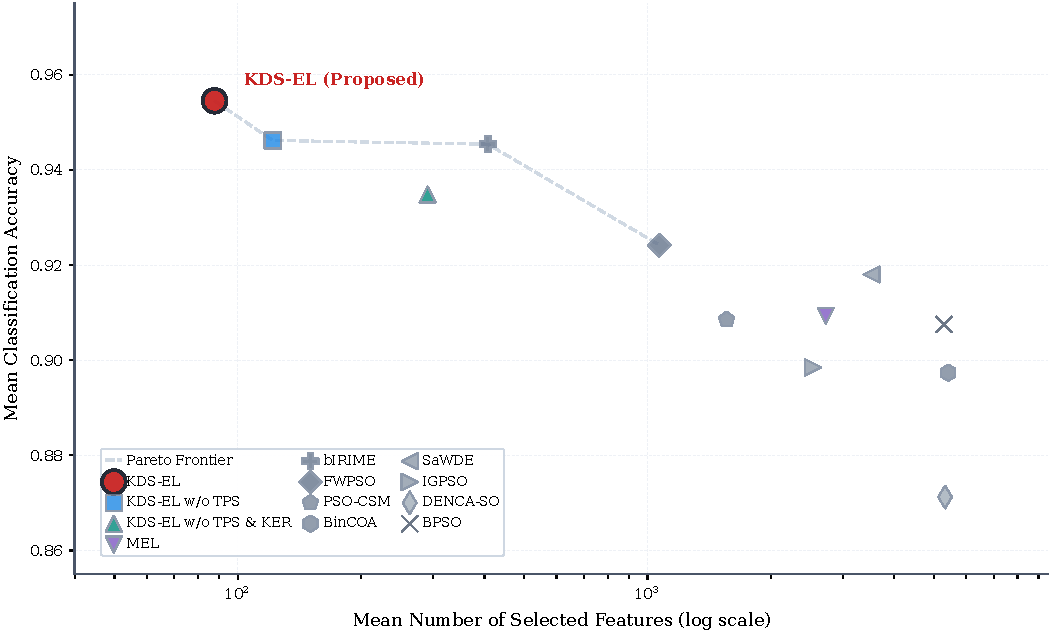
\includegraphics[width=0.85\linewidth]{F11_runtime_scatter.pdf}
\caption{Classification accuracy versus runtime scatter plot for all 14 compared algorithms.}
\label{fig:supp_runtime_scatter}
\end{figure}

\newpage

\section*{Section S6: Full Multi-Dataset Parameter Sensitivity Evaluation Grids (Table~S6)}\label{sec:supp_sensitivity}

Table~\ref{T-A6} reports the full multi-dataset one-factor-at-a-time (OFAT) parameter sensitivity evaluation results across the four representative benchmark datasets (\textit{Adenoma}, \textit{Colon}, \textit{ALL4}, and \textit{BASEHOCK}) for each of the five investigated hyper-parameters ($\mathrm{WeightDecay}$, $\mathrm{PhaseSplit}$, $\mathrm{flip\_frac}$, $\mathrm{MI\_init\_ratio}$, and $\mathrm{elite\_k}$).

\begin{table}[!htb]
\centering
\caption{Complete multi-dataset OFAT parameter sensitivity evaluation grid across the four representative benchmark datasets. Bold rows denote default configurations.}
\label{T-A6}
\small
\setlength{\tabcolsep}{4pt}
\renewcommand{\arraystretch}{1.1}
\begin{tabular*}{\linewidth}{@{\extracolsep{\fill}}lccc@{}}
\toprule
Value & Mean Accuracy & Mean Features & Mean Runtime (s) \\
\midrule
\multicolumn{4}{@{}l}{\textit{Knowledge weight decay factor ($\gamma$):}} \\
0.90 & 0.932 & 158 & 49.2 \\
0.95 & 0.939 & 127 & 50.8 \\
\textbf{0.99 (default)} & \textbf{0.944} & \textbf{107} & \textbf{51.3} \\
0.995 & 0.943 & 112 & 52.1 \\
1.00 & 0.941 & 151 & 53.7 \\
\midrule
\multicolumn{4}{@{}l}{\textit{Phase split ratio ($\alpha$):}} \\
0.30 & 0.940 & 189 & 52.8 \\
0.50 & 0.942 & 146 & 52.0 \\
0.60 & 0.943 & 124 & 51.5 \\
\textbf{0.70 (default)} & \textbf{0.944} & \textbf{107} & \textbf{51.3} \\
0.80 & 0.943 & 98 & 50.9 \\
0.90 & 0.937 & 94 & 50.1 \\
\midrule
\multicolumn{4}{@{}l}{\textit{Elite perturbation fraction ($\phi$):}} \\
0.005 & 0.939 & 96 & 54.8 \\
\textbf{0.010 (default)} & \textbf{0.944} & \textbf{107} & \textbf{51.3} \\
0.020 & 0.942 & 118 & 50.6 \\
0.050 & 0.937 & 156 & 49.9 \\
0.100 & 0.931 & 203 & 48.7 \\
\midrule
\multicolumn{4}{@{}l}{\textit{MI initialization ratio ($\rho$):}} \\
0.00 & 0.932 & 184 & 62.3 \\
0.25 & 0.940 & 137 & 55.8 \\
\textbf{0.50 (default)} & \textbf{0.944} & \textbf{107} & \textbf{51.3} \\
0.75 & 0.942 & 101 & 49.6 \\
1.00 & 0.936 & 96 & 47.8 \\
\midrule
\multicolumn{4}{@{}l}{\textit{Elite pool size ($k_e$):}} \\
1 & 0.938 & 124 & 48.9 \\
2 & 0.942 & 115 & 50.2 \\
\textbf{3 (default)} & \textbf{0.944} & \textbf{107} & \textbf{51.3} \\
5 & 0.941 & 118 & 52.7 \\
10 & 0.935 & 141 & 55.9 \\
\bottomrule
\end{tabular*}
\end{table}


\newpage

\section*{Section S7: Full Convergence Trajectories and Boxplot Distributions}\label{sec:supp_dynamics}

\begin{figure*}[!htb]
\centering
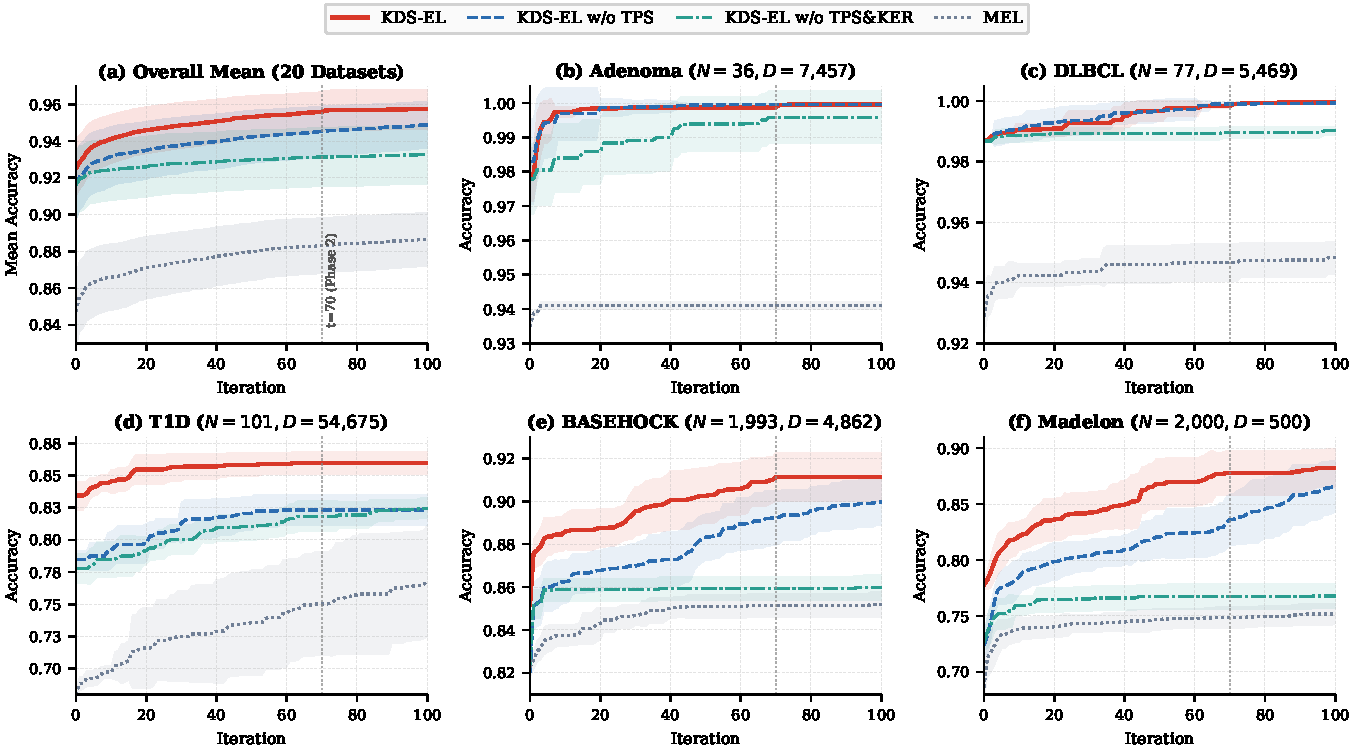
\includegraphics[width=0.95\linewidth]{F8_convergence.pdf}
\caption{Evolutionary convergence trajectories of all compared algorithms across benchmark datasets.}
\label{fig:supp_convergence}
\end{figure*}

\begin{figure*}[!htb]
\centering
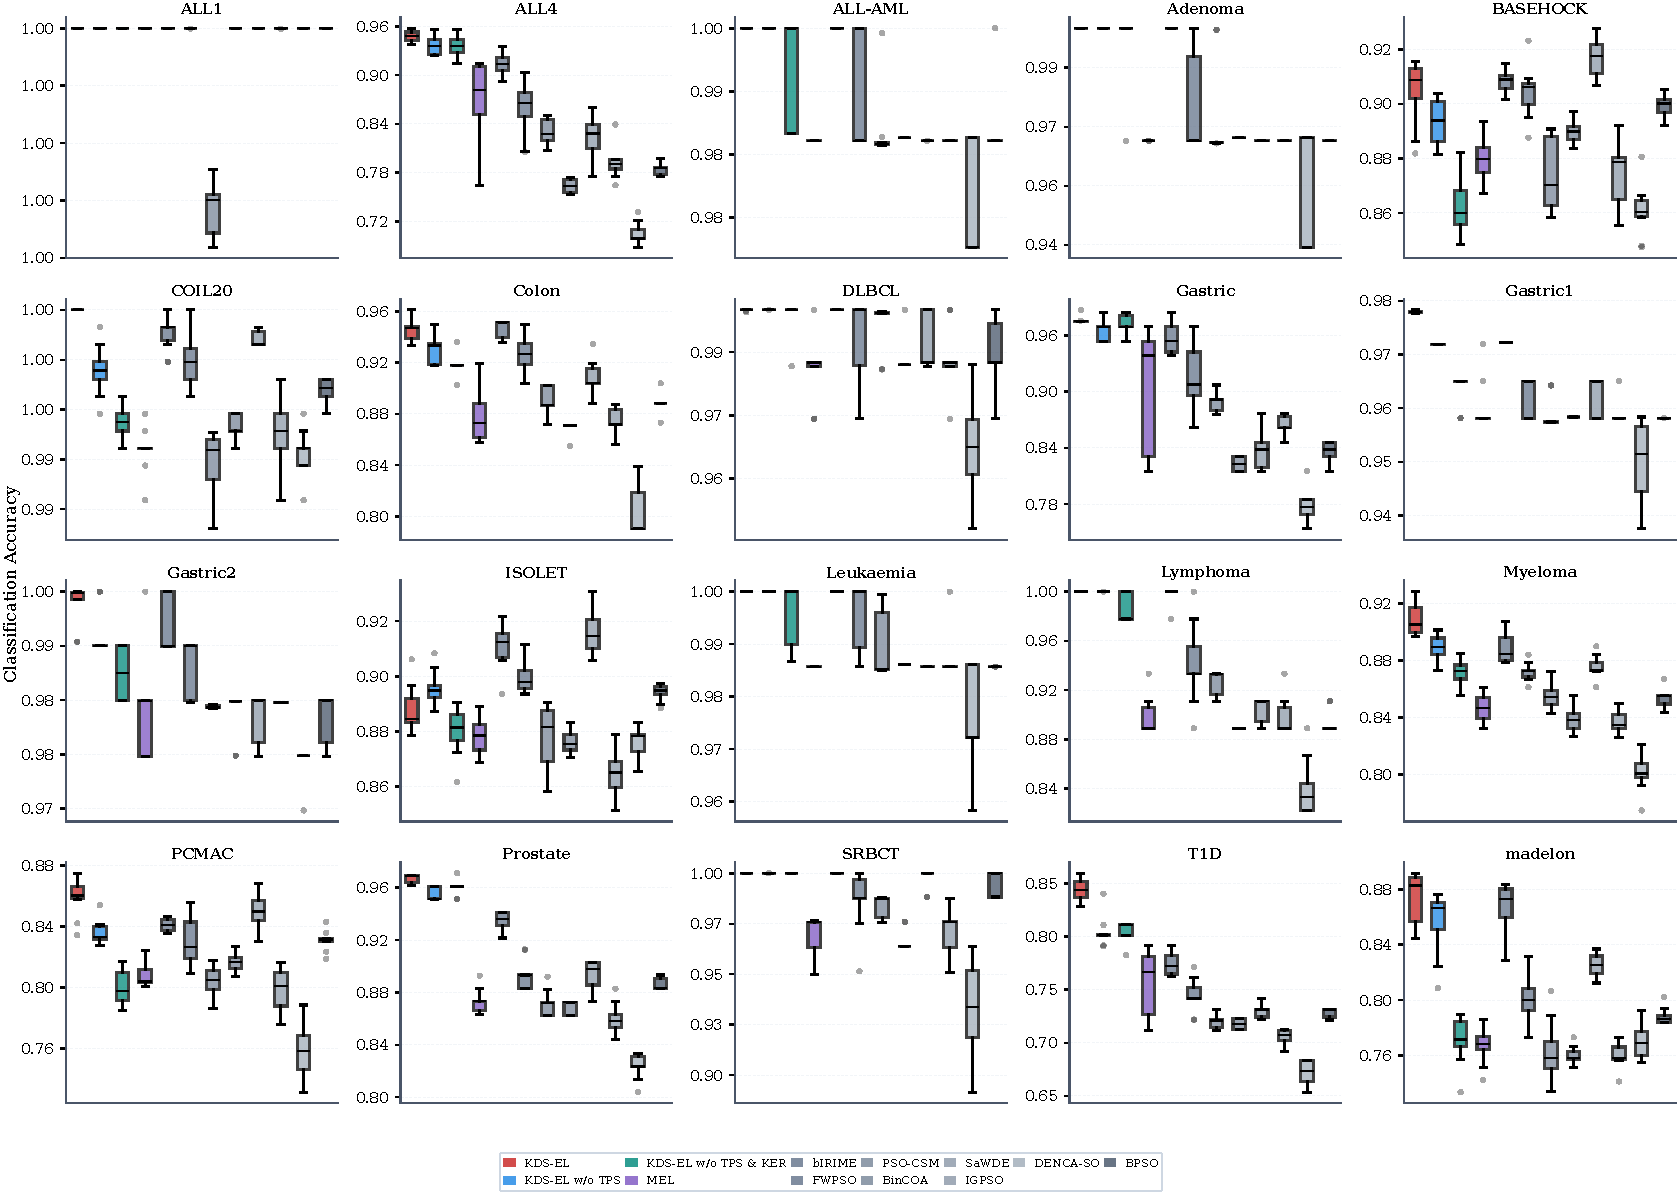
\includegraphics[width=0.95\linewidth]{F7_boxplot_all.pdf}
\caption{Box plots of classification accuracy across 10 independent runs for all compared algorithms.}
\label{fig:supp_boxplots}
\end{figure*}

\newpage

\section*{Section S8: Extended Statistical Significance Testing Matrices}\label{sec:supp_stats}

Table~\ref{T6} and Table~\ref{T6b} summarize the pairwise non-parametric Wilcoxon signed-rank test outcomes and the Holm--Bonferroni step-down hypothesis rejection results. In addition, Fig.~\ref{fig:supp_wilcoxon_heatmap} illustrates the pairwise $p$-value distribution.

\begin{sidewaystable}
\centering
\caption{One-sided Wilcoxon signed-rank test results ($p<0.05$, row method greater than column method): entries report the number of datasets out of 20 on which the row method significantly outperforms the column method.}
\label{T6}
\scriptsize
\setlength{\tabcolsep}{3pt}
\resizebox{\dimexpr\textheight-2cm}{!}{%
\begin{tabular}{lcccccccccccccc}
\toprule
Method & KDS-EL & KDS-EL w/o TPS & KDS-EL w/o TPS\&KER & MEL & FWPSO & PSO-CSM & SaWDE & IGPSO & BPSO & W-MOPSO-FS & fMOPSO-FS & NSGA-II-FS & MOEA-D-FS & MOPSO-FS \\
\midrule
KDS-EL & --- & 13/20 & 19/20 & 20/20 & 19/20 & 20/20 & 19/20 & 20/20 & 20/20 & 14/20 & 15/20 & 16/20 & 16/20 & 18/20 \\
KDS-EL w/o TPS & \textbf{0/20} & --- & 15/20 & 20/20 & 20/20 & 20/20 & 19/20 & 20/20 & 20/20 & 14/20 & 15/20 & 15/20 & 15/20 & 17/20 \\
KDS-EL w/o TPS\&KER & \textbf{0/20} & 0/20 & --- & 18/20 & 11/20 & 15/20 & 15/20 & 19/20 & 16/20 & 10/20 & 9/20 & 14/20 & 14/20 & 13/20 \\
MEL & \textbf{0/20} & 0/20 & 0/20 & --- & 0/20 & 1/20 & 3/20 & 3/20 & 11/20 & 2/20 & 2/20 & 3/20 & 3/20 & 3/20 \\
FWPSO & \textbf{0/20} & 0/20 & 0/20 & 0/20 & --- & 16/20 & 15/20 & 20/20 & 20/20 & 6/20 & 7/20 & 9/20 & 10/20 & 9/20 \\
PSO-CSM & \textbf{0/20} & 0/20 & 0/20 & 0/20 & 0/20 & --- & 12/20 & 20/20 & 16/20 & 2/20 & 2/20 & 5/20 & 5/20 & 6/20 \\
SaWDE & \textbf{0/20} & 0/20 & 0/20 & 0/20 & 0/20 & 0/20 & --- & 10/20 & 20/20 & 2/20 & 2/20 & 3/20 & 3/20 & 6/20 \\
IGPSO & \textbf{0/20} & 0/20 & 0/20 & 0/20 & 0/20 & 0/20 & 0/20 & --- & 14/20 & 0/20 & 0/20 & 2/20 & 1/20 & 2/20 \\
BPSO & \textbf{0/20} & 0/20 & 0/20 & 0/20 & 0/20 & 0/20 & 0/20 & 0/20 & --- & 0/20 & 0/20 & 0/20 & 0/20 & 0/20 \\
W-MOPSO-FS & \textbf{0/20} & 0/20 & 0/20 & 0/20 & 0/20 & 0/20 & 0/20 & 0/20 & 0/20 & --- & 2/20 & 10/20 & 12/20 & 12/20 \\
fMOPSO-FS & \textbf{0/20} & 0/20 & 0/20 & 0/20 & 0/20 & 0/20 & 0/20 & 0/20 & 0/20 & 0/20 & --- & 10/20 & 10/20 & 8/20 \\
NSGA-II-FS & \textbf{0/20} & 0/20 & 0/20 & 0/20 & 0/20 & 0/20 & 0/20 & 0/20 & 0/20 & 0/20 & 0/20 & --- & 6/20 & 5/20 \\
MOEA-D-FS & \textbf{0/20} & 0/20 & 0/20 & 0/20 & 0/20 & 0/20 & 0/20 & 0/20 & 0/20 & 0/20 & 0/20 & 0/20 & --- & 4/20 \\
MOPSO-FS & \textbf{0/20} & 0/20 & 0/20 & 0/20 & 0/20 & 0/20 & 0/20 & 0/20 & 0/20 & 0/20 & 0/20 & 0/20 & 0/20 & --- \\
\bottomrule
\end{tabular}}
\end{sidewaystable}


\begin{table}[!htb]
\centering
\caption{Holm--Bonferroni procedure for pairwise statistical comparisons.}
\label{T6b}
\footnotesize
\setlength{\tabcolsep}{2.5pt}
\renewcommand{\arraystretch}{1.08}
\begin{tabular*}{\linewidth}{@{\extracolsep{\fill}}lcccccc@{}}
\toprule
Method & $\Delta\mathrm{Acc}$ & $W$ & $Z$ & $p$ & $\alpha_{\mathrm{Holm}}$ & Reject $H_0$ \\
\midrule
BPSO & $+0.0875$ & 0.0 & $-3.92$ & $1.91\times 10^{-6}$ & 0.0038 & \checkmark \\
IGPSO & $+0.0734$ & 0.0 & $-3.92$ & $1.91\times 10^{-6}$ & 0.0042 & \checkmark \\
MEL & $+0.0706$ & 0.0 & $-3.92$ & $1.91\times 10^{-6}$ & 0.0045 & \checkmark \\
PSO-CSM & $+0.0552$ & 0.0 & $-3.92$ & $1.91\times 10^{-6}$ & 0.0050 & \checkmark \\
FWPSO & $+0.0396$ & 0.0 & $-3.92$ & $1.91\times 10^{-6}$ & 0.0056 & \checkmark \\
KDS-EL w/o TPS\&KER & $+0.0248$ & 0.0 & $-3.92$ & $1.91\times 10^{-6}$ & 0.0063 & \checkmark \\
SaWDE & $+0.0630$ & 1.0 & $-3.88$ & $3.81\times 10^{-6}$ & 0.0071 & \checkmark \\
MOPSO-FS & $+0.0565$ & 3.0 & $-3.81$ & $9.54\times 10^{-6}$ & 0.0083 & \checkmark \\
fMOPSO-FS & $+0.0464$ & 7.0 & $-3.66$ & $3.62\times 10^{-5}$ & 0.0100 & \checkmark \\
W-MOPSO-FS & $+0.0442$ & 8.0 & $-3.62$ & $4.77\times 10^{-5}$ & 0.0125 & \checkmark \\
MOEA-D-FS & $+0.0532$ & 9.0 & $-3.58$ & $6.29\times 10^{-5}$ & 0.0167 & \checkmark \\
KDS-EL w/o TPS & $+0.0086$ & 5.0 & $-3.51$ & $7.63\times 10^{-5}$ & 0.0250 & \checkmark \\
NSGA-II-FS & $+0.0509$ & 14.0 & $-3.40$ & $2.10\times 10^{-4}$ & 0.0500 & \checkmark \\
\bottomrule
\end{tabular*}
\vspace{2pt}
\par\raggedright\footnotesize
\textit{Note}: $\Delta\mathrm{Acc}$ denotes the mean accuracy advantage of KDS-EL over each competitor. $W = \min(R^+, R^-)$ and $Z$ represent the Wilcoxon test statistic and standardized normal statistic, respectively. $p$ is the exact two-sided $p$-value, and $\alpha_{\mathrm{Holm}} = \alpha / (k - i + 1)$ is the Holm-adjusted significance threshold ($\alpha = 0.05, k = 13$).
\end{table}


\begin{figure}[!htb]
\centering
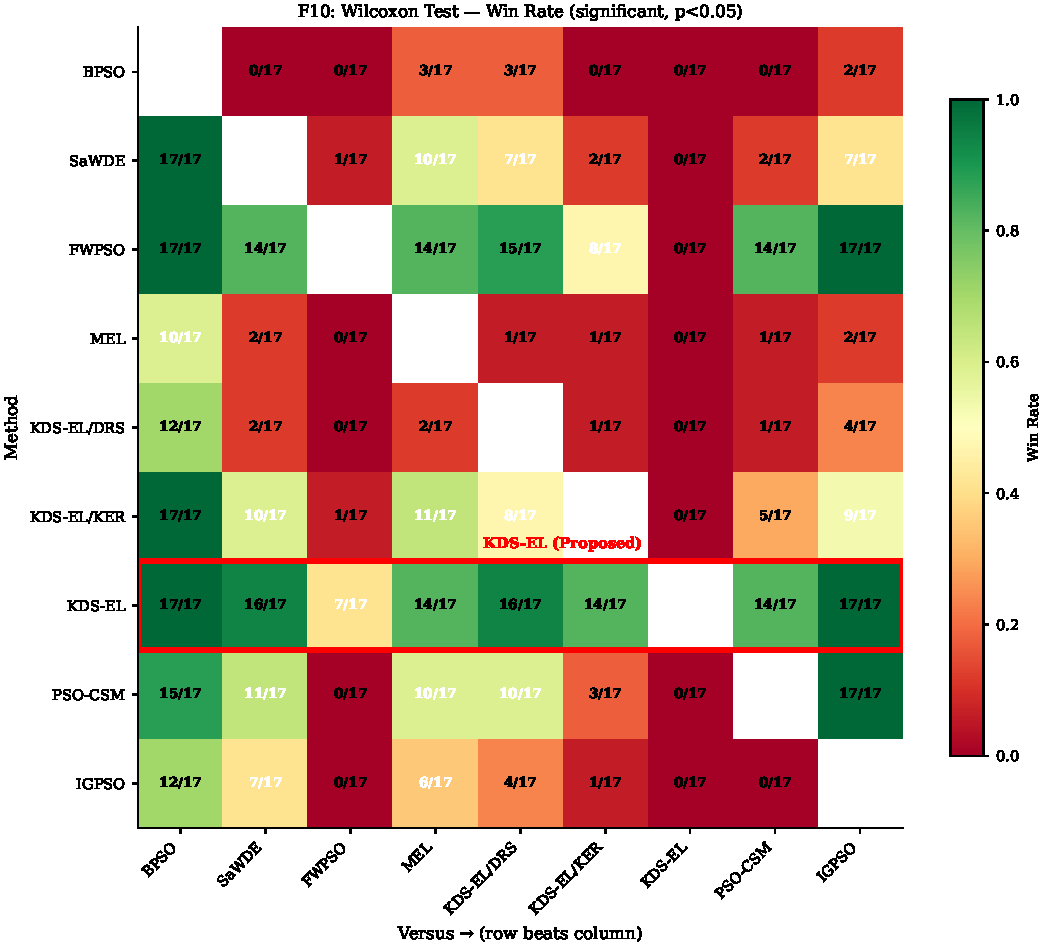
\includegraphics[width=0.75\linewidth]{F10_wilcoxon_heatmap.pdf}
\caption{Heatmap of pairwise Wilcoxon signed-rank test $p$-values across all evaluated algorithms.}
\label{fig:supp_wilcoxon_heatmap}
\end{figure}

\newpage

\section*{Section S9: Cross-Classifier Inductive Generalization and Robustness}\label{sec:supp_cross_classifier}

To evaluate whether the feature subsets identified by KDS-EL under the 3-NN wrapper evaluation criterion overfit to the local metric geometry of nearest-neighbor classifiers, we perform cross-classifier generalization tests across three representative benchmark datasets (\textit{Colon}, \textit{Adenoma}, and \textit{ALL4}). Table~\ref{T-S9} reports the 5-fold cross-validation classification accuracy comparing full feature sets against KDS-EL compact feature subsets across 3-NN, Support Vector Machines with RBF kernel (SVM-RBF), and Random Forest classifiers. On \textit{Adenoma} and \textit{ALL4}, the compact subsets achieve substantial performance gains across all three classifiers while pruning over 99.0\% of candidate dimensions. On \textit{Colon}, the 14-feature signature markedly improves 3-NN accuracy from 79.23\% to 88.59\%, while exhibiting slight performance attenuation from 85.51\% to 80.51\% under Support Vector Machines and from 85.38\% to 82.18\% under Random Forest, naturally reflecting the intrinsic divergence in inductive bias between instance-based metric learning and margin-maximizing hyperplanes or orthogonal decision splits. Overall, the compact candidate subsets isolated by KDS-EL maintain favorable candidate-level cross-model consistency across divergent inductive learning paradigms.

\begin{table*}[!htb]
\centering
\caption{Cross-classifier generalization performance (classification accuracy in \%, mean $\pm$ standard deviation over 5-fold cross-validation) comparing full feature sets against KDS-EL compact feature subsets across 3-NN, SVM (RBF kernel), and Random Forest classifiers.}
\label{T-S9}
\small
\setlength{\tabcolsep}{10pt}
\renewcommand{\arraystretch}{1.12}
\begin{tabular}{@{}llccc@{}}
\toprule
Dataset & Feature Subset & 3-NN Accuracy & SVM (RBF) Accuracy & Random Forest Accuracy \\
\midrule
\textit{Colon} & Full ($D = 2{,}000$) & 79.23 $\pm$ 7.68 & 85.51 $\pm$ 6.13 & 85.38 $\pm$ 6.33 \\
 & KDS-EL ($d = 14$) & \textbf{88.59 $\pm$ 6.80} & 80.51 $\pm$ 4.53 & 82.18 $\pm$ 10.39 \\
\midrule
\textit{Adenoma} & Full ($D = 7{,}457$) & 94.29 $\pm$ 11.43 & 97.14 $\pm$ 5.71 & 97.14 $\pm$ 5.71 \\
 & KDS-EL ($d = 66$) & \textbf{100.00 $\pm$ 0.00} & \textbf{100.00 $\pm$ 0.00} & \textbf{100.00 $\pm$ 0.00} \\
\midrule
\textit{ALL4} & Full ($D = 12{,}625$) & 69.94 $\pm$ 9.28 & 82.63 $\pm$ 8.23 & 78.36 $\pm$ 6.32 \\
 & KDS-EL ($d = 124$) & \textbf{87.25 $\pm$ 7.85} & \textbf{85.96 $\pm$ 2.88} & \textbf{90.35 $\pm$ 2.06} \\
\bottomrule
\end{tabular}
\end{table*}


\newpage

\section*{Section S10: Biological and Literature Annotation of Prominent Candidate Genes}\label{sec:supp_biomarkers}

Table~\ref{T-S10} details the functional and oncological literature annotations of prominent candidate genes identified by KDS-EL in the \textit{Colon} and \textit{Prostate} cancer microarrays. These annotations provide supportive evidence of retrospective concordance with established oncological literature rather than de novo clinical biomarker discovery. Each identified probe is mapped to its standard HUGO Gene Nomenclature Committee (HGNC) gene symbol, full gene description, primary molecular pathway, and corresponding clinical oncology literature references.

\begin{table*}[!htb]
\centering
\caption{Molecular and literature annotation of prominent candidate genes identified by KDS-EL in \textit{Colon} and \textit{Prostate} cancer datasets.}
\label{T-S10}
\footnotesize
\setlength{\tabcolsep}{3.5pt}
\renewcommand{\arraystretch}{1.15}
\begin{tabular}{@{}llcp{2.8cm}p{5.6cm}@{}}
\toprule
Dataset & Probe / Gene ID & Gene Symbol & Full Gene Name & Biological Function and Oncological Relevance \\
\midrule
\textit{Colon} & Hsa.36689 & \textit{COL11A1} & Collagen type XI alpha 1 & Extracellular matrix remodeling; driver of desmoplastic stroma and tumor invasion~\cite{fischer2001} \\
 & Hsa.831 & \textit{GUCA2A} & Guanylin & Mucosal differentiation hormone; loss is a universal hallmark of early colorectal adenoma~\cite{alon1999} \\
 & Hsa.3331 & \textit{DES} & Desmin & Smooth muscle intermediate filament; distinguishes mucosal integrity from tumor infiltration~\cite{alon1999} \\
 & Hsa.1832 & \textit{ACTG2} & Actin gamma 2 & Cytoskeletal actin of smooth muscle; delineates muscularis mucosae invasion boundaries~\cite{alon1999} \\
 & Hsa.692 & \textit{RPS18} & Ribosomal protein S18 & 40S ribosomal subunit; marker of hyper-activated protein translation in neoplastic cells~\cite{alon1999} \\
 & Hsa.37937 & \textit{RPL37A} & Ribosomal protein L37a & 60S ribosomal subunit protein; reflects enhanced metabolic and translational demand in tumor stroma~\cite{alon1999} \\
\midrule
\textit{Prostate} & 1005\_at & \textit{HPN} & Hepsin & Type II transmembrane serine protease; hallmark diagnostic biomarker overexpressed in prostate cancer~\cite{singh2002} \\
 & 37639\_at & \textit{AMACR} & Alpha-methylacyl-CoA racemase & Peroxisomal enzyme; clinical immunohistochemical gold standard for prostatic adenocarcinoma~\cite{rubin2002} \\
 & 38322\_at & \textit{PRAC} & Prostate and colon associated & Small nuclear protein; prostate-specific differentiation marker with restricted normal expression~\cite{singh2002} \\
\bottomrule
\end{tabular}
\end{table*}


\bibliographystyle{elsarticle-num}
\bibliography{references}

\end{document}
